\documentclass[11pt,a4paper]{article}

\usepackage[T1]{fontenc}
\usepackage[utf8]{inputenc}
\usepackage[margin=2.5cm]{geometry}
\usepackage{graphicx}
\usepackage{amsmath}
\usepackage{amssymb}
\usepackage{booktabs}
\usepackage{algorithm}
\usepackage{algpseudocode}
\usepackage{caption}
\usepackage{subcaption}
\usepackage{hyperref}
\usepackage{url}
\usepackage{float}

\title{MONET -- Supplementary Material \\ \large Algorithm, Hyperparameters,
Sensitivity Analysis, and Node-Coverage Bounds}
\author{Julian Hatzky \and Thomas Bartz-Beielstein \and A.~E.\ Eiben \and Anil Yaman}
\date{}

\hypersetup{
  pdftitle={MONET Supplementary: Algorithm, Hyperparameters, Sensitivity Analysis},
  pdfauthor={Hatzky, Bartz-Beielstein, Eiben, Yaman},
  colorlinks=true, linkcolor=blue, urlcolor=blue, citecolor=blue
}

\begin{document}
\maketitle

\noindent
This document accompanies the MONET paper \emph{``Multi-Task Optimization
over Networks of Tasks''} (Hatzky et al., 2026) and the code repository
at \url{https://github.com/ju2ez/MONET}. It collects the full MONET
pseudocode (main loop + the two learning subroutines), the hyperparameter
reference used throughout the experiments, the per-domain sensitivity
analysis (SHAP beeswarm plots and SPOT-tuned configurations), and the
coupon-collector bounds that justify the $10^{6}$-evaluation budget.

\tableofcontents
\bigskip

\section{MONET Algorithm}\label{sec:algorithm}

Algorithm~\ref{alg:monet} gives the main MONET loop;
Algorithms~\ref{alg:individual} and~\ref{alg:social} detail the two
learning subroutines invoked from it.

\begin{algorithm}[H]
\caption{MONET}\label{alg:monet}
\begin{algorithmic}[1]
\Require Task set $T=\{\boldsymbol{\tau}_1,\dots,\boldsymbol{\tau}_n\}$,
  fitness function~$f$, task distance~$d$
\Require Budget~$E$, init fraction~$K_{\text{init}}$,
  neighborhood size~$N$, selection strategy \Call{Select}{$\cdot$},
  probability~$p_{\text{ind}}$
\Ensure Network $\mathcal{N}$ mapping each task to its best solution
\Statex
\State $\mathcal{N}[\boldsymbol{\tau}] \gets \emptyset$ for all
       $\boldsymbol{\tau} \in T$ \Comment{empty network}
\For{each $\boldsymbol{\tau}_i \in T$} \Comment{build $k$-NN task graph}
    \State $\mathrm{Nb}(\boldsymbol{\tau}_i) \gets N$ nearest tasks
           under~$d$
\EndFor
\Statex
\For{$i \gets 1$ \textbf{to} $K_{\text{init}}$}
     \Comment{random initialisation}
    \State $\boldsymbol{\tau} \gets \Call{RandomTask}{T}$
    \State $\mathbf{x} \sim \mathcal{U}(p_{\min}, p_{\max})$
    \State $f_x \gets f(\mathbf{x}, \boldsymbol{\tau})$
    \If{$\mathcal{N}[\boldsymbol{\tau}] = \emptyset$ \textbf{or}
        $f_x \geq \mathcal{N}[\boldsymbol{\tau}].\text{fitness}$}
        \Comment{elitist update}
        \State $\mathcal{N}[\boldsymbol{\tau}] \gets (\mathbf{x}, f_x)$
    \EndIf
\EndFor
\Statex
\State $e \gets K_{\text{init}}$ \Comment{main loop}
\While{$e < E$}
    \State $\boldsymbol{\tau} \gets \Call{RandomTask}{T}$
          \Comment{sample focal task}
    \If{$\mathrm{rand}() < p_{\text{ind}}$}
           \Comment{individual learning}
        \State \Call{IndividualLearning}{$\boldsymbol{\tau}, \mathcal{N}$}
               \Comment{Alg.~\ref{alg:individual}}
        \State $e \gets e + 1$
    \Else \Comment{social learning}
        \State $\boldsymbol{\tau}_j \gets
               \Call{Select}{\mathrm{Nb}(\boldsymbol{\tau})}$
               \Comment{pick one neighbor}
        \If{$\boldsymbol{\tau}_j \neq \text{nil}$}
             \Comment{skip if no graph neighbor exists}
            \State \Call{SocialLearning}{$\boldsymbol{\tau},
                     \boldsymbol{\tau}_j, \mathcal{N}$}
                   \Comment{Alg.~\ref{alg:social}}
            \State $e \gets e + 1$
        \EndIf
    \EndIf
\EndWhile
\State \Return $\mathcal{N}$
\end{algorithmic}
\end{algorithm}

\paragraph{Individual learning.}
When individual learning is selected, the current elite at node
$\boldsymbol{\tau}_i$ is mutated independently of any neighbor. If no
solution exists at the node, a random solution is drawn from
$\mathcal{U}(p_{\min}, p_{\max})$ and evaluated. Otherwise, Gaussian
mutation with standard deviation $\sigma_m$ scaled by the parameter
range is applied. The offspring replaces the current elite only if its
fitness is at least as high.

\begin{algorithm}[H]
\caption{Individual Learning}\label{alg:individual}
\begin{algorithmic}[1]
\Require Task $\boldsymbol{\tau}$, network $\mathcal{N}$,
         bounds $p_{\min}, p_{\max}$, mutation std $\sigma_m$
\Ensure Updated $\mathcal{N}[\boldsymbol{\tau}]$
\If{$\mathcal{N}[\boldsymbol{\tau}] = \emptyset$}
    \Comment{initialise empty node}
    \State $\mathbf{x} \sim \mathcal{U}(p_{\min}, p_{\max})$
           \Comment{random solution}
    \State $\mathcal{N}[\boldsymbol{\tau}] \gets (\mathbf{x},\,
           f(\mathbf{x}, \boldsymbol{\tau}))$
    \State \Return
\EndIf
\State $\mathbf{x} \gets \mathcal{N}[\boldsymbol{\tau}].\text{solution}$
       \Comment{current elite}
\State $\boldsymbol{\epsilon} \sim \mathcal{N}(\mathbf{0},\,
       \sigma_m (p_{\max} - p_{\min}))$
       \Comment{Gaussian perturbation}
\State $\mathbf{y} \gets \text{clip}(\mathbf{x} +
       \boldsymbol{\epsilon},\; p_{\min},\; p_{\max})$
       \Comment{mutant offspring}
\State $f_y \gets f(\mathbf{y}, \boldsymbol{\tau})$
\If{$f_y \geq \mathcal{N}[\boldsymbol{\tau}].\text{fitness}$}
    \Comment{elitist replacement}
    \State $\mathcal{N}[\boldsymbol{\tau}] \gets (\mathbf{y}, f_y)$
\EndIf
\end{algorithmic}
\end{algorithm}

\paragraph{Social learning.}
When social learning is selected, the current elite is recombined with
a solution drawn from a neighboring node. If the current node is empty,
the neighbor's solution is copied as an initial seed (or a random
solution is used when no neighbor has a solution). Recombination is
performed via Simulated Binary Crossover (SBX; Deb \& Agrawal, 1995)
with distribution index $\eta_c=10$ (Deb, 2001). As with individual
learning, the offspring replaces the elite only upon improvement.

\begin{algorithm}[H]
\caption{Social Learning}\label{alg:social}
\begin{algorithmic}[1]
\Require Task $\boldsymbol{\tau}$, neighbor task $\boldsymbol{\tau}_j$,
         archive $\mathcal{A}$, bounds $p_{\min}, p_{\max}$
\Ensure Updated $\mathcal{A}[\boldsymbol{\tau}]$
\If{$\mathcal{A}[\boldsymbol{\tau}] = \emptyset$}
    \Comment{initialise empty node}
    \If{$\mathcal{A}[\boldsymbol{\tau}_j] \neq \emptyset$}
        \State $\mathbf{x} \gets
               \mathcal{A}[\boldsymbol{\tau}_j].\text{solution}$
               \Comment{copy from neighbor}
    \Else
        \State $\mathbf{x} \sim \mathcal{U}(p_{\min}, p_{\max})$
               \Comment{random fallback}
    \EndIf
    \State $\mathcal{A}[\boldsymbol{\tau}] \gets (\mathbf{x},\,
           f(\mathbf{x}, \boldsymbol{\tau}))$
    \State \Return
\EndIf
\If{$\mathcal{A}[\boldsymbol{\tau}_j] = \emptyset$}
    \State \Return \Comment{no valid neighbor solution}
\EndIf
\State $\mathbf{y} \gets \text{SBX}\bigl(
       \mathcal{A}[\boldsymbol{\tau}].\text{solution},\;
       \mathcal{A}[\boldsymbol{\tau}_j].\text{solution},\;
       \eta_c\!=\!10\bigr)$
       \Comment{crossover}
\State $\mathbf{y} \gets \text{clip}(\mathbf{y},\,
       p_{\min},\, p_{\max})$
\State $f_y \gets f(\mathbf{y}, \boldsymbol{\tau})$
\If{$f_y \geq \mathcal{A}[\boldsymbol{\tau}].\text{fitness}$}
    \Comment{elitist replacement}
    \State $\mathcal{A}[\boldsymbol{\tau}] \gets (\mathbf{y}, f_y)$
\EndIf
\end{algorithmic}
\end{algorithm}

\section{MONET Hyperparameter Descriptions}\label{sec:hyperparameters}

Table~\ref{tab:monet-hyperparams} summarises the four hyperparameters
varied in the sensitivity analysis. All other algorithmic parameters
(mutation operator, crossover operator, initialisation strategy) are
held fixed throughout.

\begin{table}[H]
\centering
\caption{MONET hyperparameters and their roles.}
\label{tab:monet-hyperparams}
\renewcommand{\arraystretch}{1.3}
\small
\begin{tabular}{@{}p{2.6cm}p{2.2cm}p{9.4cm}@{}}
\toprule
\textbf{Parameter} & \textbf{Values} & \textbf{Description} \\
\midrule
$p_\text{ind}$ &
0, 0.3, 0.5, 0.7, 1 &
Probability that a given evaluation step performs
\emph{individual learning} (mutation of the focal task's own elite)
rather than \emph{social learning} (crossover with a neighbor's
elite). At $p_\text{ind}=0$ only social learning occurs; at
$p_\text{ind}=1$ only individual learning occurs. \\
\addlinespace
strategy &
random, best\_fitness &
Neighbor selection strategy during social learning.
\texttt{random}: uniform random selection among all neighbors.
\texttt{best\_fitness}: deterministically select the neighbor with
the highest current fitness. \\
\addlinespace
neighborhood &
random, closest, distance\_prop. &
Method for constructing the neighbor set of each task.
\texttt{closest}: the $N$ nearest tasks by Euclidean distance in task
space.
\texttt{random}: $N$ tasks sampled uniformly at random (sorted by
similarity after sampling).
\texttt{distance\_proportional}: $N$ tasks sampled \emph{without
replacement} with probability proportional to task-space similarity
$s(\boldsymbol{\tau}_i, \boldsymbol{\tau}_j) =
  1/(1 + \lVert \boldsymbol{\tau}_i - \boldsymbol{\tau}_j \rVert)$;
this softly biases the neighborhood toward nearby tasks while
retaining a chance of including distant ones. \\
\addlinespace
neighbor\_pct. &
1\%, 5\%, 10\% &
Fraction of the total task set used as the neighborhood size
$N = \lceil \texttt{neighbor\_percentage} \cdot |\mathcal{V}| \rceil$.
For instance, with 5\,000 tasks and 5\%, each task has $N=250$
neighbors. Controls graph sparsity: lower values yield sparser graphs
with more localised knowledge transfer. \\
\bottomrule
\end{tabular}
\end{table}

\section{Detailed Sensitivity Analysis}\label{sec:sensitivity}

This section provides per-domain SHAP beeswarm plots and the
SPOT-tuned hyperparameter configurations that complement the global
analysis in the main paper.

\subsection{Per-Domain SHAP Analysis}

Figures~\ref{fig:shap-archery}--\ref{fig:shap-hexapod} show the SHAP
beeswarm plots for the four domains. Each point represents one MONET
run; its horizontal position indicates the SHAP value (contribution to
the predicted metric), and its colour encodes the feature value
(red = high, blue = low).

In all domains, $p_\text{ind}$ exhibits the strongest effect: high
values of $p_\text{ind}$ (more individual learning) consistently
decrease predicted fitness, corroborating the global finding that
social learning is the primary driver of performance. The remaining
parameters show smaller, more task-specific effects.

\begin{figure}[H]
    \centering
    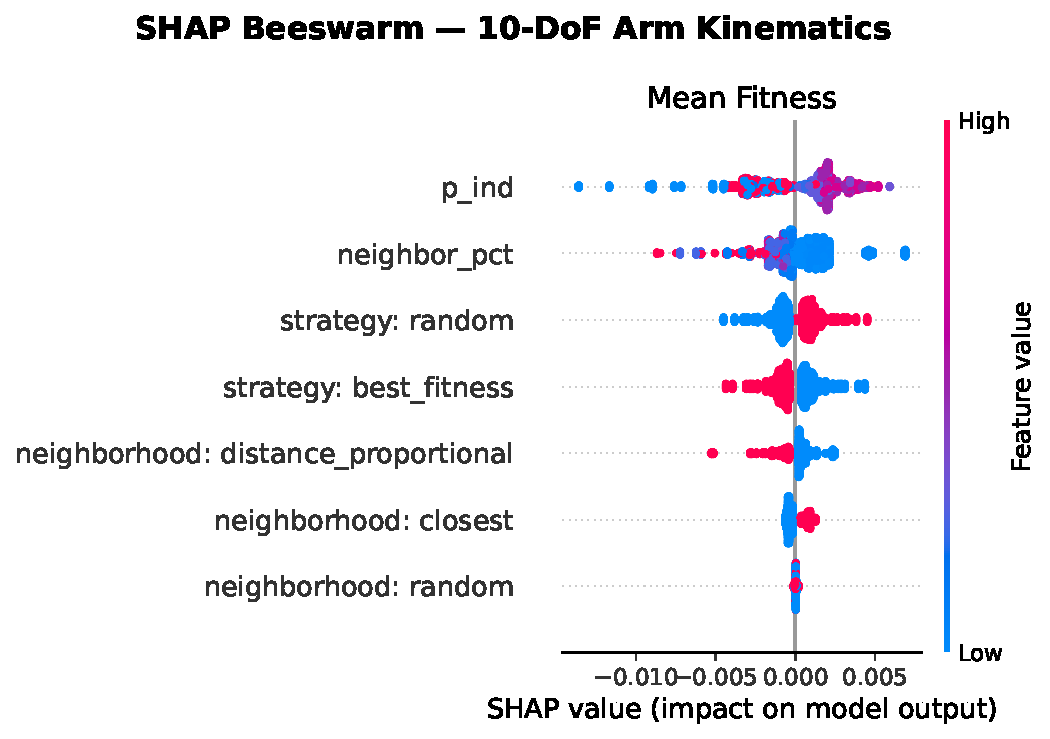
\includegraphics[width=1\linewidth]{figs/monet_hyperparam_importance_arm.pdf}
    \caption{SHAP beeswarm plot for the 10-DoF Arm domain. Each row
    is a hyperparameter; each dot is a MONET run. Colour indicates the
    feature value (red = high, blue = low); horizontal position
    indicates the SHAP value.}
    \label{fig:shap-arm}
\end{figure}

\begin{figure}[H]
    \centering
    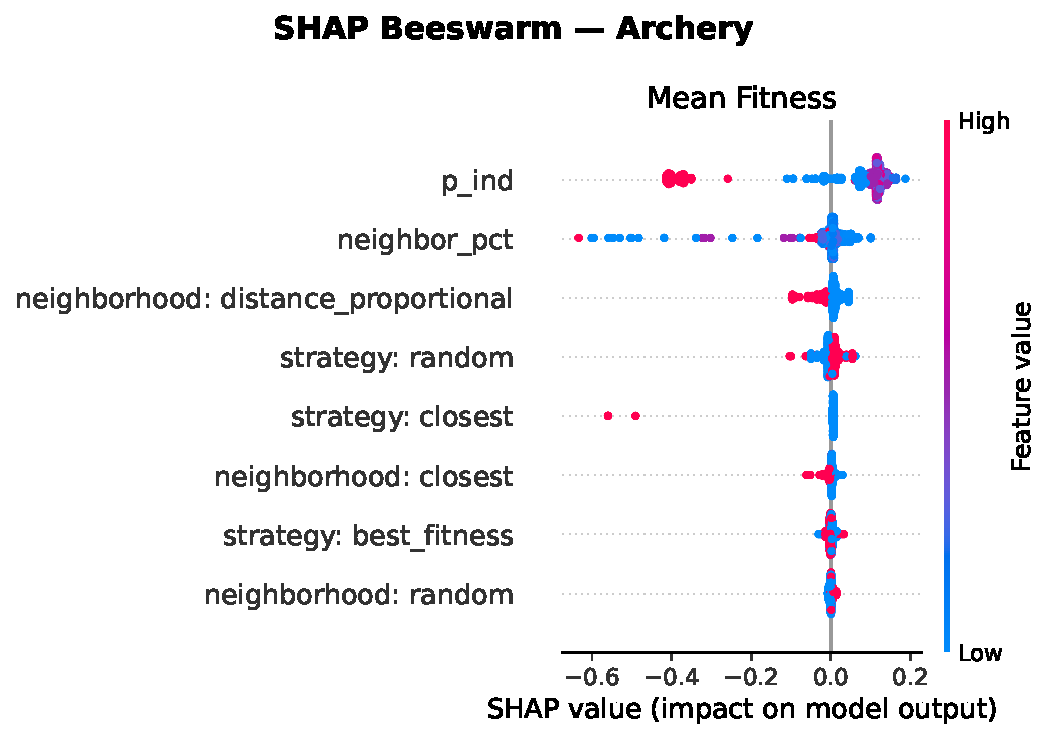
\includegraphics[width=1\linewidth]{figs/monet_hyperparam_importance_archery.pdf}
    \caption{SHAP beeswarm plot for the Archery domain. Panels as in
    Figure~\ref{fig:shap-arm}.}
    \label{fig:shap-archery}
\end{figure}

\begin{figure}[H]
    \centering
    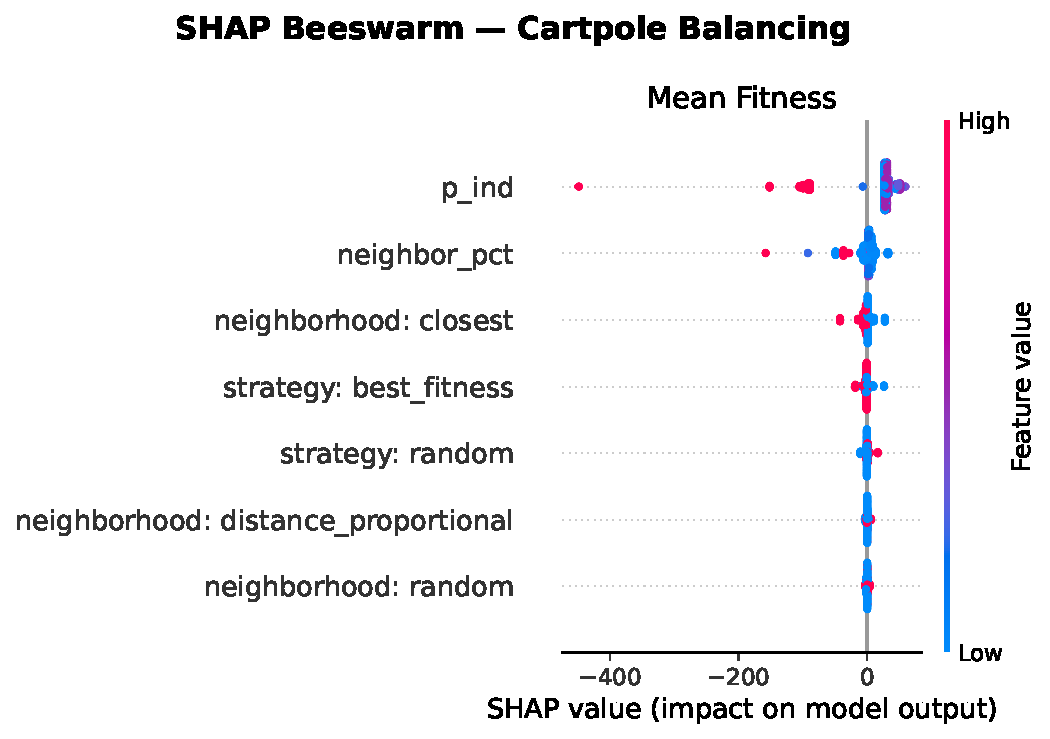
\includegraphics[width=1\linewidth]{figs/monet_hyperparam_importance_cartpole.pdf}
    \caption{SHAP beeswarm plot for the Cartpole Balancing domain.
    Panels as in Figure~\ref{fig:shap-arm}.}
    \label{fig:shap-cartpole}
\end{figure}

\begin{figure}[H]
    \centering
    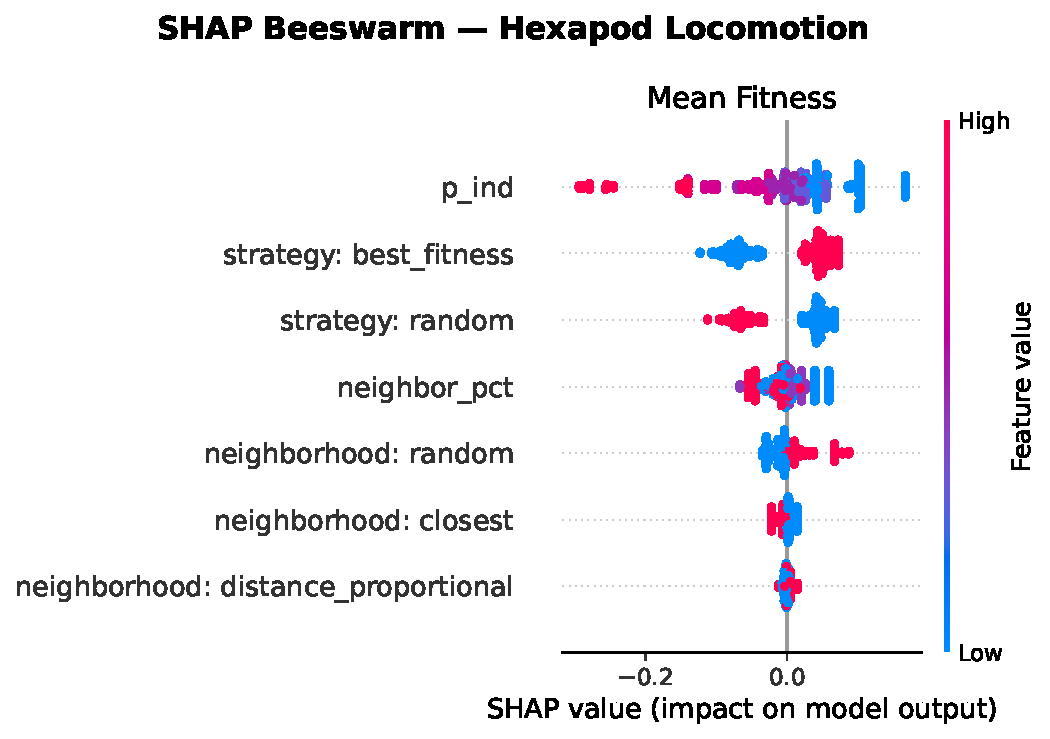
\includegraphics[width=1\linewidth]{figs/monet_hyperparam_importance_hexapod.pdf}
    \caption{SHAP beeswarm plot for the Hexapod Locomotion domain.
    Panels as in Figure~\ref{fig:shap-arm}.}
    \label{fig:shap-hexapod}
\end{figure}

\subsection{SPOT-Tuned Configurations}

Table~\ref{tab:spot-configs} lists the per-domain configurations found
by the SPOT hyperparameter tuner (Bartz-Beielstein et al., 2010, 2024,
2026). The surrogate-model-based tuning loop is implemented in
\texttt{hpt\_spot.py} in the repository root and drives
\texttt{run\_algorithms.py} as a black-box evaluator.

\begin{table}[H]
\centering
\caption{SPOT-tuned MONET configurations per domain.}
\label{tab:spot-configs}
\small
\begin{tabular}{@{}lllcc@{}}
\toprule
\textbf{Domain} & \textbf{strategy} & \textbf{neighborhood}
    & $p_\text{ind}$ & \textbf{neighbor\_pct.} \\
\midrule
Arm      & random        & closest  & 0.3 & 1\% \\
Archery  & best\_fitness & closest  & 0.0 & 2\% \\
Cartpole & best\_fitness & random   & 0.5 & 1\% \\
Hexapod  & best\_fitness & random   & 0.0 & 1\% \\
\bottomrule
\end{tabular}
\end{table}

\section{Node Coverage Guarantees Under Random Sampling}
\label{sec:coupon}

If we draw at each evaluation step a random node and perform an
action, we may ask how many evaluations are required so that we
visit each of the $\nu$ nodes at least once with high certainty.
This is the classical \emph{coupon collector's problem}
(Feller, 1968). Writing $M$ for the number of draws, the expected
number of steps needed to visit all $\nu$ nodes at least once is
\[
\mathbb{E}[M] = \nu H_\nu
             = \nu \left( \ln \nu + \gamma
                   + O\!\left(\frac{1}{\nu}\right) \right),
\]
where $H_\nu$ is the $\nu$-th harmonic number and
$\gamma \approx 0.57721$ is the Euler-Mascheroni constant.

\bigskip
Beyond the expectation, one may also ask for a high-probability
guarantee. Using the asymptotic limit for the coupon-collector
completion time, the probability that all nodes have been visited by
draw
\[
M = \nu(\ln \nu + c)
\]
converges to
\[
\mathbb{P}\bigl(M \le \nu(\ln \nu + c)\bigr) \approx e^{-e^{-c}}.
\]
To achieve at least $99\%$ probability of having visited all nodes,
we solve for~$c$:
\[
\begin{aligned}
e^{-e^{-c}} &= p, \\[4pt]
\ln\!\left(e^{-e^{-c}}\right) &= \ln(p), \\[4pt]
-e^{-c} &= \ln(p), \\[4pt]
\text{For } p = 0.99:\quad
c &= -\ln\!\bigl(-\ln(0.99)\bigr)
     \approx 4.60015 \approx \ln(100).
\end{aligned}
\]
Since each node is selected independently with probability
$\tfrac{1}{\nu}$ at every draw, the visit count of any particular
node over $M$ draws follows a Binomial distribution,
\[
X_i \sim \mathrm{Binomial}\!\left(M, \tfrac{1}{\nu}\right),
\qquad
\mathbb{E}[X_i] = \frac{M}{\nu}.
\]

We evaluate four environments with differing numbers of distinct
tasks and a fixed draw budget of $M=1{,}000{,}000$ evaluations:

\begin{table}[H]
\centering
\caption{Coupon-collector bounds for the four benchmark environments
with $M=1{,}000{,}000$ total evaluations.}
\label{tab:coupon-collector}
\begin{tabular}{@{}lrrrr@{}}
\toprule
Environment & $\nu$ & $\mathbb{E}[M]$ & $M_{0.99}$
   & $\mathbb{E}[X_i]$ \\
\midrule
Hexapod                  & 2\,000 & 16\,356 & 24\,412 & 500 \\
Archery / Arm / Cartpole & 5\,000 & 45\,472 & 65\,612 & 200 \\
\bottomrule
\end{tabular}
\end{table}

\section*{References (selected)}

\begin{itemize}\small
    \item Bartz-Beielstein, T.\ (2010). \emph{SPOT: An R Package for
    Automatic and Interactive Tuning of Optimization Algorithms by
    Sequential Parameter Optimization}.
    \href{https://arxiv.org/abs/1006.4645}{arXiv:1006.4645} \textbullet{}
    \href{https://doi.org/10.48550/arXiv.1006.4645}
    {doi:10.48550/arXiv.1006.4645}.
    \item Bartz-Beielstein, T., Zaefferer, M., and Rehbach, F.\ (2024).
    \emph{Hyperparameter Tuning for Machine and Deep Learning with R:
    A Practical Guide}. Springer.
    \href{https://doi.org/10.1007/978-981-19-5170-1}
    {doi:10.1007/978-981-19-5170-1}.
    \item Bartz-Beielstein, T.\ (2026). \emph{Optimization with
    SpotOptim}.
    \href{https://arxiv.org/abs/2604.13672}{arXiv:2604.13672} \textbullet{}
    \href{https://pypi.org/project/spotoptim/}{pypi.org/project/spotoptim}.
    \item Deb, K.\ and Agrawal, R.\ B.\ (1995). \emph{Simulated Binary
    Crossover for Continuous Search Space}. \emph{Complex Systems}
    9(2):115--148.
    \href{https://www.complex-systems.com/abstracts/v09_i02_a02/}
    {complex-systems.com/abstracts/v09\_i02\_a02}.
    \item Deb, K.\ (2001). \emph{Multi-Objective Optimization Using
    Evolutionary Algorithms}. Wiley. ISBN~978-0-471-87339-6.
    \item Feller, W.\ (1968). \emph{An Introduction to Probability
    Theory and Its Applications}, Vol.~1, 3rd ed.\ Wiley.
    \item Hutter, F., Hoos, H., and Leyton-Brown, K.\ (2014).
    \emph{An Efficient Approach for Assessing Hyperparameter
    Importance}. In \emph{Proc.\ ICML 2014}, PMLR 32:754--762.
    \href{https://proceedings.mlr.press/v32/hutter14.html}
    {proceedings.mlr.press/v32/hutter14}.
    \item Lundberg, S.~M., Erion, G., Chen, H., DeGrave, A., Prutkin, J.\ M.,
    Nair, B., Katz, R., Himmelfarb, J., Bansal, N., and Lee, S.-I.\
    (2020). \emph{From Local Explanations to Global Understanding with
    Explainable AI for Trees}. \emph{Nature Machine Intelligence}
    2(1):56--67.
    \href{https://doi.org/10.1038/s42256-019-0138-9}
    {doi:10.1038/s42256-019-0138-9}.
    \item Lundberg, S.~M.\ and Lee, S.-I.\ (2017). \emph{A Unified
    Approach to Interpreting Model Predictions}. In \emph{Advances in
    Neural Information Processing Systems} 30 (NeurIPS 2017).
    \href{https://arxiv.org/abs/1705.07874}{arXiv:1705.07874} \textbullet{}
    \href{https://papers.nips.cc/paper/2017/hash/8a20a8621978632d76c43dfd28b67767-Abstract.html}
    {NeurIPS proceedings}.
    \item Mann, H.~B.\ and Whitney, D.~R.\ (1947). \emph{On a Test of
    Whether one of Two Random Variables is Stochastically Larger than
    the Other}. \emph{Annals of Mathematical Statistics}
    18(1):50--60.
    \href{https://doi.org/10.1214/aoms/1177730491}
    {doi:10.1214/aoms/1177730491}.
    \item Holm, S.\ (1979). \emph{A Simple Sequentially Rejective
    Multiple Test Procedure}. \emph{Scandinavian Journal of
    Statistics} 6(2):65--70.
    \href{https://www.jstor.org/stable/4615733}{jstor:4615733}.
\end{itemize}

\end{document}
